\section{Eficiência}

\subsection{Protocolo utilizado}

O protocolo implementado baseia-se num sistema \textit{Stop-and-Wait ARQ}. O seu nome advém da natureza do comportamento do emissor e do recetor:
\begin{itemize}
    \item \textbf{Stop-and-Wait} porque o emissor espera pela resposta do recetor a cada trama
    \item \textbf{ARQ ou Automatic Repeat Request} porque o recetor automaticamente requer a repetição do envio da trama se esta contiver erros ou não corresponder ao esperado
\end{itemize}

\subsubsection{Funcionamento do protocolo}

\begin{enumerate}
    \item O emissor envia uma trama e espera pela resposta do recetor
    \item \begin{itemize}
        \item Se o recetor receber a trama que espera, envia uma mensagem de acknowledgement ao emissor 'ACK'
        \item Caso receba uma trama que não corresponde à esperada ou que contenha erros,  envia uma mensagem de rejeição, de modo a que o emissor reenvie a mensagem 'NACK'
    \end{itemize}
    \item \begin{itemize}
        \item Recomeça o processo para a próxima trama ou
        \item Reenvia a trama 
    \end{itemize}
\end{enumerate}

\subsubsection{Mecanismos de deteção de erros}

\paragraph{Através da numeração das tramas} com os valores 0 ou 1, o recetor é capaz de distinguir se a trama recebida é aquela que se pretende ou se é apenas uma retransmissão ou se houve um lapso da trama.

\paragraph{BCC1 e BCC2} são dois componentes da trama cuja função é detetar um eventual bit flip no cabeçalho ou conteúdo da trama, respetivamente.

\subsection{Análise de Dados}

De modo a entender de que forma afetam a performance do protocolo alguns dos seus parâmetros, foi executada uma recolha e análise de dados.

O nosso protocolo baseia-se num sistema \textit{Stop-and-Wait ARQ}. 

\subsubsection{Definições}
\paragraph{Descrições}
\begin{itemize}
    \item \textbf{S} - eficiência
    \item \textbf{FER} ou $\boldsymbol{p_e}$ - probabilidade de erro numa trama
    \item \textbf{R} ou $\boldsymbol{T_f}$ - débito recebido
    \item $\boldsymbol{T_prop}$ - tempo de propagação da trama
\end{itemize}

\paragraph{Formulas}
\begin{itemize}
    \item $\boldsymbol{a} = \frac{T_prop}{T_f}$
    \item \textbf{Sem erros:} $\boldsymbol{S} = \frac{T_f}{T_prop + T_f + T_prop} = \frac{1}{2a}$
    \item \textbf{Com erros:} $\boldsymbol{S} = \frac{1 - p_e}{2a}$
\end{itemize}


\subsubsection{Gráficos}

Para a recolha de dados, os valores por defeito são:

\begin{itemize}
    \item $Baudrate = 38400$
    \item $Framesize = 150 B$
    \item $T_prop = 0$
    \item $FER = 0$
\end{itemize}

\paragraph{FER}

Os resultados da nossa análise indicam-nos que as fórmulas a cima descritas, no que toca à influência dos erros na trama na eficiência do protocolo, estão corretos. Estas conclusões são suportadas pelo gráfico abaixo.

\begin{center}
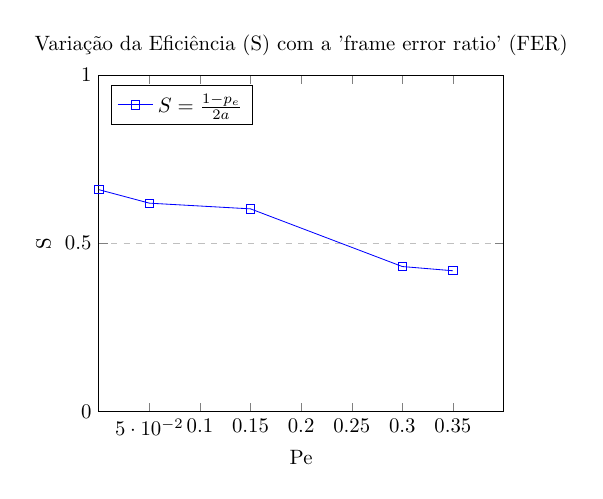
\begin{tikzpicture}[scale = 0.75]
    \begin{axis}[
        title={Variação da Eficiência (S) com a 'frame error ratio' (FER)},
        xlabel={Pe},
        ylabel={S},
        xmin=0, xmax=0.4,
        ymin=0, ymax=1,
        xtick={0.05,0.1,0.15,0.20,0.25,0.30,0.35},
        ytick={0,0.5,1,1.5,2,2.5,3},
        legend pos=north west,
        ymajorgrids=true,
        grid style=dashed,
    ]
    
    \addplot[
        color=blue,
        mark=square,
        ]
        coordinates {
        (0,0.659451659)(0.05,0.619241192)(0.15,0.602266737)(0.30,0.43072573)(0.35,0.418191801)
        };
        \legend{$\boldsymbol{S} = \frac{1 - p_e}{2a}$}
    \end{axis}
    
\end{tikzpicture}
\end{center}

Como a regressão dos dados formou uma função linear, estes vão de encontro à fórmula prevista. A linearidade da função não é muito definida devido ao curto tamanho da amostra, que foi recolhida em laboratório em tempo limitado.


\paragraph{Tempo de propagação}

O próximo gráfico mostra a variação da eficiência consoante o tempo de propagação, o que valida as fórmulas no sentido de que S varia em proporcionalidade inversa com a.
\begin{center}
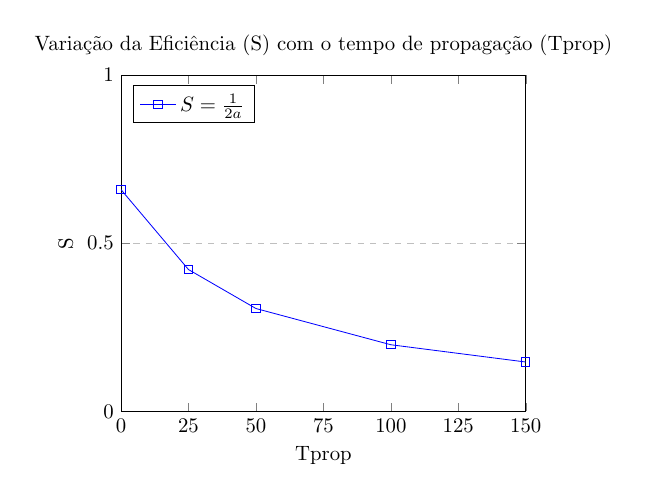
\begin{tikzpicture}[scale = 0.75]
    \begin{axis}[
        title={Variação da Eficiência (S) com o tempo de propagação (Tprop)},
        xlabel={Tprop},
        ylabel={S},
        xmin=0, xmax=150,
        ymin=0, ymax=1,
        xtick={0,25,50,75,100,125,150},
        ytick={0,0.5,1,1.5,2,2.5,3},
        legend pos=north west,
        ymajorgrids=true,
        grid style=dashed,
    ]
    
    \addplot[
        color=blue,
        mark=square,
        ]
        coordinates {
        (0,0.659451659)(25,0.421820196)(50,0.305890228)(100,0.198144294)(150,0.146784865)
        };
        \legend{$\boldsymbol{S} = \frac{1}{2a}$}
    \end{axis}
    
\end{tikzpicture}
\end{center}

\paragraph{Baudrate}

\begin{center}
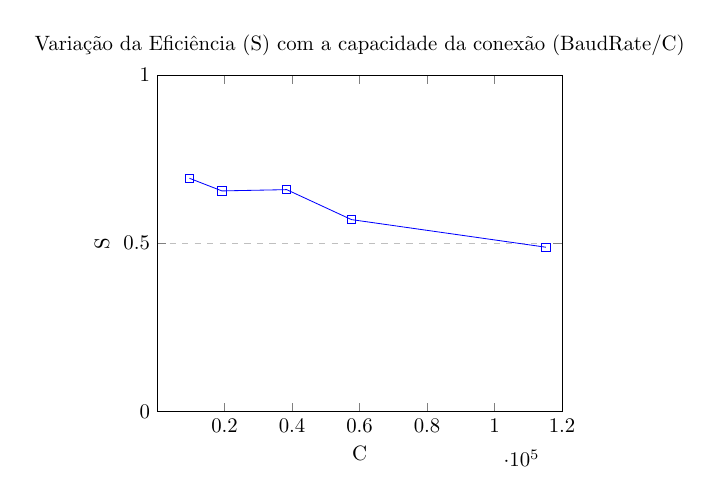
\begin{tikzpicture}[scale = 0.75]
    \begin{axis}[
        title={Variação da Eficiência (S) com a capacidade da conexão (BaudRate/C)},
        xlabel={C},
        ylabel={S},
        xmin=50, xmax=120000,
        ymin=0, ymax=1,
        xtick={0,20000,40000,60000,80000,100000,120000},
        ytick={0,0.5,1,1.5,2,2.5,3},
        legend pos=north west,
        ymajorgrids=true,
        grid style=dashed,
    ]
    
    \addplot[
        color=blue,
        mark=square,
        ]
        coordinates {
        (9600,0.693106848)(19200,0.655667145)(38400,0.659451659)(57600,0.570323225)(115200,0.488247863)
        };
        
    \end{axis}
    
\end{tikzpicture}
\end{center}

O gráfico permite-nos concluir que a eficiência do protocolo diminui com o aumento da capacidade da ligação de dados. Estima-se que esta viesse a subir até um dado valor. No entanto, infelizmente, essa subida não está representada na gama de valores que foram recolhidos.

\newpage
\paragraph{Tamanho de trama}

\begin{center}
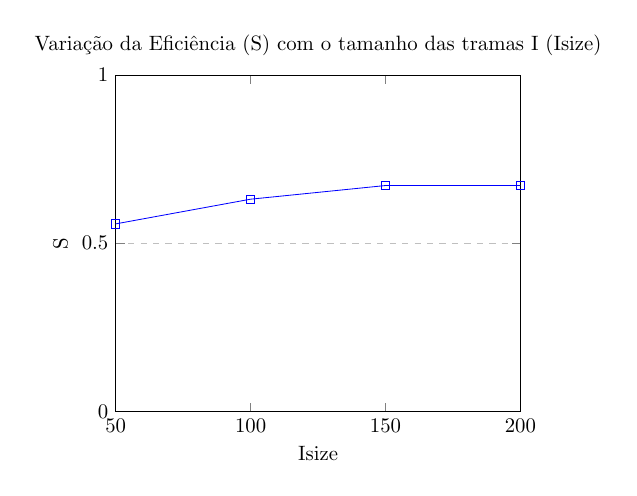
\begin{tikzpicture}[scale = 0.75]
    \begin{axis}[
        title={Variação da Eficiência (S) com o tamanho das tramas I (Isize)},
        xlabel={Isize},
        ylabel={S},
        xmin=50, xmax=200,
        ymin=0, ymax=1,
        xtick={0,50,100,150,200},
        ytick={0,0.5,1,1.5,2,2.5,3},
        legend pos=north west,
        ymajorgrids=true,
        grid style=dashed,
    ]
    
    \addplot[
        color=blue,
        mark=square,
        ]
        coordinates {
        (50,0.557589068)(100,0.631041149)(150,0.671663727)(200,0.671663727)
        };
        
    \end{axis}
    
\end{tikzpicture}
\end{center}

Por último conclui-se que o tamanho das tramas beneficia a eficiência mas apenas até um certo ponto, começando a estancar por volta dos 150 bytes.


    

